\newcommand{\assignmentDate}{December 2nd, 2019}

% Add title
%Institute
\begin{tabular*}{\hsize}{l@{\extracolsep{\fill}} r}
	\textsc{Technical University of Berlin}		 \hfill&								 	\\
	Faculty II - Mathematics and Natural Sciences\hfill&									\\
	Institute of Mathematics 					 \hfill&									\\
	Dr. D. Peschka, A. Selahi 		 			 \hfill&									\\
\end{tabular*}

% Title
\begin{center}
	\textbf{\Large{\courseName}}\\
	\vspace{7pt}
	\large{Homework \currentAssignment}\\
	\smallskip
	\normalsize{Submitted on \assignmentDate}
\end{center}

% Group table
\begin{center}
	\vspace{-8pt}
	\begin{tabular}{l c r}
		by \textbf{\groupNumber}		    &	 			  &		 								\\
		\hline
		\texttt{Kagan Atci} 			    & \texttt{338131} & \texttt{Physical Engineering, M.Sc.}\\
		\texttt{Navneet Singh }		 	    & \texttt{380443} & \texttt{Scientific Computing, M.Sc.}\\ 
		\texttt{Daniel V. Herrmannsdoerfer} & \texttt{412543} & \texttt{Scientific Computing, M.Sc.}\\ 
		\hline
	\end{tabular}
\end{center}

% EXERCISE 1
% --------------------------------------------------------------------------------------------------------------------
\addExercise{1}{Ex1}

%
% ----------------
\addSubExercise{a}

%
% ----------------
\addSubExercise{b}

%
% ----------------
\addSubExercise{c}

%
% EXERCISE 2
% --------------------------------------------------------------------------------------------------------------------
\addExercise{2}{Ex2}
%
% ----------------
\addSubExercise{a}

%
% ----------------
\addSubExercise{b}

%
% ----------------
\addSubExercise{c}

%
% EXERCISE 3
% --------------------------------------------------------------------------------------------------------------------
\addExercise{3}{Ex3}

\addSubExercise{a}
Please refer to the online submitted \texttt{a06e03getPDE.py} file.

\addSubExercise{b and c}

The grid size was empirically defined as $N = 20 + 10\sqrt{\varepsilon^{-1}}$.

\begin{figure}[H]
	\centering
	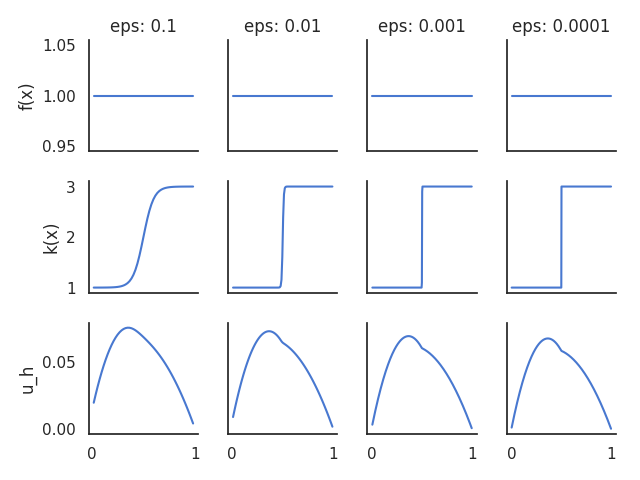
\includegraphics[width=0.68\textwidth]{a06e03plot.png}
	\caption{Functions $f(x)$, $k(x)$ and $u_h$ evaluated for $\varepsilon = 0.1, 0.01, 0.001, 0.0001$}
	\label{fig:a06e03plot}
\end{figure}

The function $k(x)$ will behave as a Heaviside step function for $\varepsilon \to 0$.